\documentclass[11pt,a4paper]{article}
\usepackage{fontspec}
\setmainfont[Path=fonts/,FontIndex=7,BoldFont=AvenirNext.ttc,BoldFeatures={FontIndex=2},ItalicFont=AvenirNext.ttc,ItalicFeatures={FontIndex=4},BoldItalicFont=AvenirNext.ttc,BoldItalicFeatures={FontIndex=3}]{AvenirNext.ttc}
\setsansfont[Path=fonts/,FontIndex=7,BoldFont=AvenirNext.ttc,BoldFeatures={FontIndex=2},ItalicFont=AvenirNext.ttc,ItalicFeatures={FontIndex=4},BoldItalicFont=AvenirNext.ttc,BoldItalicFeatures={FontIndex=3}]{AvenirNext.ttc}
\newfontfamily\heavy[Path=fonts/,FontIndex=2]{AvenirNext.ttc}
\setmonofont[Path=fonts/,BoldFont=JetBrainsMono-Bold.ttf,ItalicFont=JetBrainsMono-Italic.ttf,Contextuals=NoAlternate,Ligatures=NoCommon]{JetBrainsMono-Regular.ttf}
\usepackage{xcolor,graphicx,tikz,booktabs,tabularx,listings,amsmath}
\usetikzlibrary{arrows.meta,positioning}
\definecolor{paper}{HTML}{FFFFFF}
\definecolor{ink}{HTML}{252525}
\definecolor{teal}{HTML}{252525}
\definecolor{orange}{HTML}{777777}
\definecolor{wash}{HTML}{EAEAEA}
\definecolor{quiet}{HTML}{666666}
\definecolor{lightink}{HTML}{D0D0D0}
\definecolor{codepaper}{HTML}{F6F6F4}
\lstset{language=Python,basicstyle=\ttfamily\fontsize{9.5}{13}\selectfont\color{ink},keywordstyle=\bfseries\color{ink},commentstyle=\itshape\color{quiet},stringstyle=\color{ink},showstringspaces=false,columns=fullflexible,keepspaces=true,breaklines=true,breakatwhitespace=true,numbers=none,upquote=true,aboveskip=8pt,belowskip=6pt}
\hyphenpenalty=4000
\emergencystretch=3em
% The same two-line navigation and fine rule as the reference, without a candy motif.
\newcommand{\guideheader}[2]{\begin{tikzpicture}[remember picture,overlay]
\node[anchor=north west,inner sep=0,text width=176mm] at ([xshift=16mm,yshift=-7mm]current page.north west) {\fontsize{8.5}{10}\selectfont\color{quiet}#1};
\node[anchor=north west,inner sep=0,text width=176mm] at ([xshift=16mm,yshift=-11.5mm]current page.north west) {\heavy\fontsize{10}{12}\selectfont\color{ink}#2};
\draw[lightink,line width=.4pt] ([xshift=16mm,yshift=-17mm]current page.north west)--([xshift=192mm,yshift=-17mm]current page.north west);
\end{tikzpicture}}

\usepackage[a4paper,left=16mm,right=18mm,top=24mm,bottom=19mm,headheight=14pt]{geometry}
\usepackage{fancyhdr,enumitem,hyperref}
\hypersetup{colorlinks=true,linkcolor=teal,urlcolor=teal}
\setlength{\parindent}{0pt}
\setlength{\parskip}{7pt}
\setlist{nosep,leftmargin=1.4em}
\usepackage{needspace,colortbl}
\lstdefinestyle{numbered}{numbers=left,numberstyle=\ttfamily\fontsize{7.5}{13}\selectfont\color{lightink},numbersep=10pt,xleftmargin=24pt}
\pagestyle{fancy}\fancyhf{}
\fancyhead[C]{\guideheader{Lesson 2 · Dice Combinations and Grid Paths}{Worksheet Answers · \nouppercase{\leftmark}}}
\fancyfoot[L]{\fontsize{8}{10}\selectfont\color{quiet}LESSON 2 / Dice Combinations and Grid Paths}
\fancyfoot[R]{\fontsize{9}{11}\selectfont\color{quiet}\thepage}
\renewcommand{\headrulewidth}{0pt}
\newcommand{\topic}[2]{\clearpage\markboth{#2}{}{\color{quiet}\fontsize{9}{12}\selectfont\textbf{#1}}\par{\heavy\fontsize{19}{23}\selectfont\raggedright #2\par}\vspace{5pt}}
\newcommand{\topicflow}[2]{\par\Needspace{20\baselineskip}\bigskip\markboth{#2}{}{\color{quiet}\fontsize{9}{12}\selectfont\textbf{#1}}\par{\heavy\fontsize{19}{23}\selectfont\raggedright #2\par}\vspace{5pt}}
\newcommand{\labeltext}[1]{{\color{teal}\textbf{#1}}\par}
\makeatletter
\newsavebox{\qbox}
\newenvironment{qblock}[1][0.6]{\def\qlimit{#1}\par\setbox\qbox\vbox\bgroup\hsize\linewidth\color@begingroup}{\par\color@endgroup\egroup
  \ifdim\dimexpr\ht\qbox+\dp\qbox\relax>\qlimit\textheight\relax\unvbox\qbox\else\box\qbox\fi\par}
\makeatother
\newcommand{\qtopic}[2]{{\color{quiet}\fontsize{9}{12}\selectfont\textbf{#1}}\par{\heavy\fontsize{19}{23}\selectfont\raggedright #2\par}\vspace{5pt}}
\begin{document}\color{ink}\fontsize{10.5}{13}\selectfont
\thispagestyle{empty}\pagecolor{white}\null
\begin{tikzpicture}[remember picture,overlay]
\node[anchor=north west,inner sep=0,text width=174mm] at ([xshift=18mm,yshift=-22mm]current page.north west)
{\heavy\fontsize{9}{12}\selectfont ALGORITHMS\quad /\quad LESSON 02\quad /\quad WORKSHEET ANSWERS};
\node[anchor=north west,inner sep=0,text width=174mm] at ([xshift=18mm,yshift=-39mm]current page.north west)
{\heavy\fontsize{43}{47}\selectfont\raggedright\spaceskip=.25em Dice and\\Grid Paths\par};
\node[anchor=north west,inner sep=0,text width=174mm] at ([xshift=18mm,yshift=-80mm]current page.north west)
{\fontsize{19}{25}\selectfont Worked answers, tables and complete code.};
\node[anchor=north west,inner sep=0,text width=150mm] at ([xshift=18mm,yshift=-97mm]current page.north west)
{\fontsize{12}{16}\selectfont Check each answer against your own working.\\Follow the question IDs from the worksheet.};
\node[anchor=center,inner sep=0] at ([xshift=105mm,yshift=-167mm]current page.north west)
{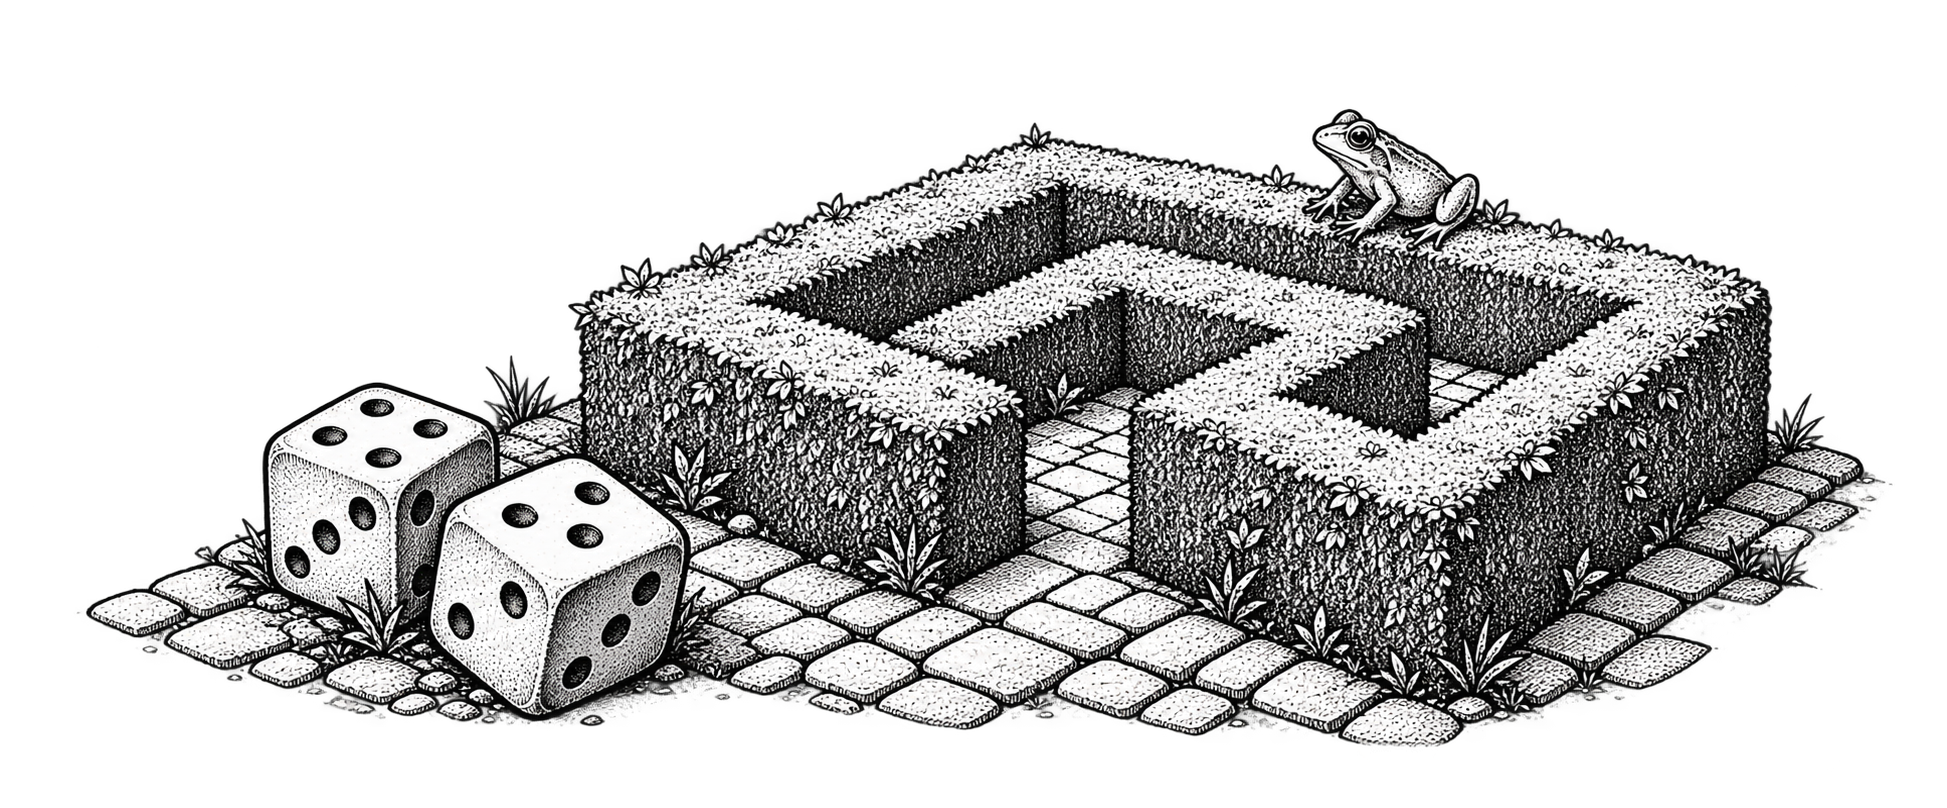
\includegraphics[width=174mm,height=94mm,keepaspectratio]{assets/cover.png}};
\node[anchor=north west,inner sep=0,text width=174mm] at ([xshift=18mm,yshift=-224mm]current page.north west)
{\fontsize{12}{16}\selectfont Questions appear in worksheet order.\\Alternative correct solutions are welcome.};
\node[anchor=west,inner sep=0] at ([xshift=18mm,yshift=-269mm]current page.north west)
{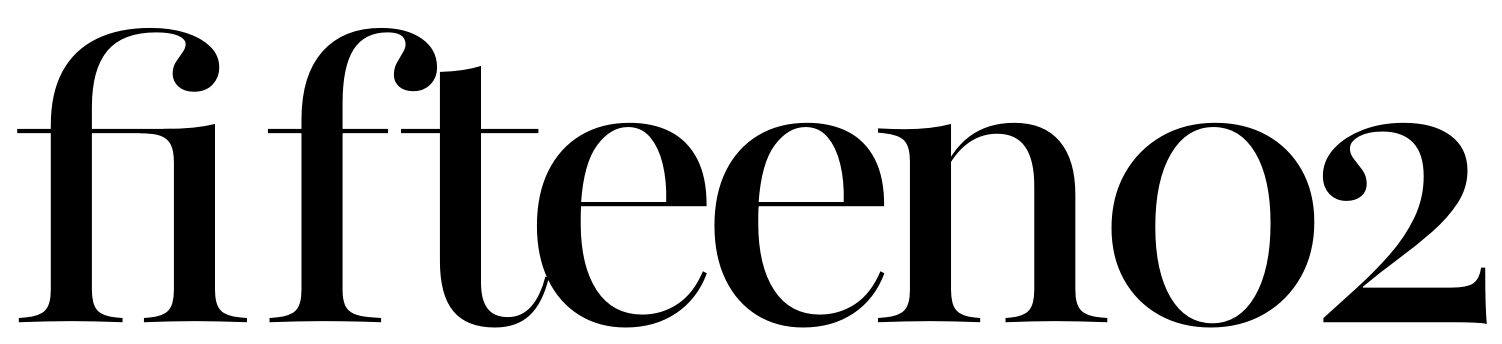
\includegraphics[width=43mm]{assets/logo.png}};
\node[anchor=east,inner sep=0] at ([xshift=192mm,yshift=-269mm]current page.north west)
{
\includegraphics[width=62mm]{assets/julians-pathfinder-monochrome.pdf}};
\end{tikzpicture}\clearpage
\topic{KEEP BESIDE YOUR WORK}{The route and the rules}
\textbf{Our route}\par Count ordered dice sequences by their final number. Try recursion, save repeated answers, then fill a table. Then see how six reused entries reduce Dice memory from O(n) to O(1), with an optional running sum. Afterwards count grid paths by their final move. The full Dice table remains useful for learning; the buffer is a memory improvement.\par\medskip
\textbf{Dice rules · L2-02 to L2-08}\par Choose any finite ordered sequence of values from 1 to 6. Count sequences whose total is exactly the target n. There is no fixed number of throws and no probability calculation. [1, 2] and [2, 1] are different sequences. For L2-07 only, allow 1, 2 and 3.\par\medskip
\textbf{Large counts}\par The final iterative dice and grid programs return the remainder after dividing the count by 1,000,000,007. Python writes this as \texttt{count \% 1\_000\_000\_007}. Small examples on these sheets are below that number, so their counts are unchanged. L2-06 explains why taking remainders during the calculation is valid.\par\medskip
\textbf{Grid rules · L2-09 to L2-14}\par The grid has n rows and n columns, numbered from 0. A dot means an open cell; a star means a blocked cell. Start at row 0, column 0. Reach row n - 1, column n - 1 using moves of one cell right or one cell down. A path may never enter a blocked cell.\par\medskip
\textbf{Names used in the questions}\par \texttt{ways[total]} stores the number of sequences whose sum is that total. \texttt{paths[r][c]} stores the number of paths to row r, column c. The indices identify a total or a cell; the stored values count sequences or paths. A recursive function answers the same question by asking about smaller totals or earlier cells.\par\medskip
\textbf{Using these answers.} Each question and its supplied diagram or table appear before the answer. Completed tables, and answer diagrams where the question has one, follow the worked answer. The IDs match the worksheet; answer pages have their own page numbers. Each program is printed in full once, with imports, line numbers and a small check; a later question that uses the same program names the page where it appears and gives its own check. An optional question remains optional here.\par\bigskip{\color{lightink}\hrule height .4pt}\bigskip\par\markboth{Recall: what are we storing?}{}\begin{qblock}\begin{qblock}[0.95]
\qtopic{L2-01}{Recall: what are we storing?}
{\small\color{quiet}Dice: count ordered sequences}\par\medskip
\textbf{Question.} In staircase, what does ways[4] = 5 mean? In Frog, what does best[4] = 30 mean? Which problem adds and which takes a minimum?

\par\medskip\textbf{Worked answer.} There are 5 routes to step 4. The cheapest Frog route to stone 4 costs 30. Staircase adds counts from separate groups; Frog takes the minimum of competing total costs.

\end{qblock}
\end{qblock}\par\medskip{\color{lightink}\hrule height .4pt}\bigskip
\par\markboth{A total of three}{}\begin{qblock}\begin{qblock}[0.95]
\qtopic{L2-02}{A total of three}
{\small\color{quiet}Dice: count ordered sequences}\par\medskip
\textbf{Question.} List every ordered sequence of numbers from 1 to 6 whose sum is exactly 3. What happens to sequences containing a 4, 5 or 6?

\par\medskip\textbf{Worked answer.} The four sequences are [3], [1, 2], [2, 1] and [1, 1, 1]. A sequence containing 4, 5 or 6 already exceeds the target. We count valid sequences rather than simulate random throws.

\end{qblock}
\end{qblock}\par\medskip{\color{lightink}\hrule height .4pt}\bigskip
\par\markboth{Six possible last numbers}{}\begin{qblock}\begin{qblock}[0.95]
\qtopic{L2-03}{Six possible last numbers}
{\small\color{quiet}Dice: count ordered sequences}\par\medskip
\textbf{Question.} Let ways[total] count ordered sequences of values 1 to 6 whose sum is that total. Explain ways[0] = 1. For target 4, group sequences by their last number and add the earlier counts. Copy your L2-02 count into total 3, then fill totals 5, 6 and 7 in the table.

\textbf{Table supplied with the question.}\par\par\medskip \begingroup\small\setlength{\tabcolsep}{4pt}\renewcommand{\arraystretch}{1.35}\begin{tabularx}{\linewidth}{>{\raggedright\arraybackslash}l>{\raggedright\arraybackslash}X>{\raggedright\arraybackslash}X>{\raggedright\arraybackslash}X>{\raggedright\arraybackslash}X>{\raggedright\arraybackslash}X>{\raggedright\arraybackslash}X>{\raggedright\arraybackslash}X>{\raggedright\arraybackslash}X}\toprule\textbf{Total} & \textbf{0} & \textbf{1} & \textbf{2} & \textbf{3} & \textbf{4} & \textbf{5} & \textbf{6} & \textbf{7}\\\midrule
ways[total] & 1 & 1 & 2 & ? & ? & ? & ? & ?\\
\bottomrule\end{tabularx}\endgroup\par\medskip 
\par\medskip\textbf{Worked answer.} The empty sequence is the one sequence with total 0. For total 4, final numbers 1, 2, 3 and 4 give counts 4 + 2 + 1 + 1 = 8. Totals 5 and 6 give 16 and 32. Total 7 uses totals 6 through 1: 32 + 16 + 8 + 4 + 2 + 1 = 63.

\textbf{Completed table.}\par\par\medskip \begingroup\small\setlength{\tabcolsep}{4pt}\renewcommand{\arraystretch}{1.35}\begin{tabularx}{\linewidth}{>{\raggedright\arraybackslash}l>{\raggedright\arraybackslash}X>{\raggedright\arraybackslash}X>{\raggedright\arraybackslash}X>{\raggedright\arraybackslash}X>{\raggedright\arraybackslash}X>{\raggedright\arraybackslash}X>{\raggedright\arraybackslash}X>{\raggedright\arraybackslash}X}\toprule\textbf{Total} & \textbf{0} & \textbf{1} & \textbf{2} & \textbf{3} & \textbf{4} & \textbf{5} & \textbf{6} & \textbf{7}\\\midrule
ways[total] & 1 & 1 & 2 & 4 & 8 & 16 & 32 & 63\\
\bottomrule\end{tabularx}\endgroup\par\medskip 
For target 4, a final 1 leaves target 3 with 4 sequences; a final 2 leaves target 2 with 2; a final 3 leaves target 1 with 1; a final 4 leaves target 0 with 1. A final 5 or 6 is impossible. Total 5 adds 8 + 4 + 2 + 1 + 1 = 16; total 6 adds 16 + 8 + 4 + 2 + 1 + 1 = 32.

\end{qblock}
\end{qblock}\par\medskip{\color{lightink}\hrule height .4pt}\bigskip
\par\markboth{Dice: recursion, then caching}{}\begin{qblock}\begin{qblock}[0.95]
\qtopic{L2-04}{Dice: recursion, then caching}
{\small\color{quiet}Dice: count ordered sequences}\par\medskip
\textbf{Question.} Write dice\_slow(n) recursively to count ordered sequences of faces 1 to 6 with total n. Trace target 4. Then write dice\_cached(n), adding a cache: which input identifies a repeated question? Use the uncached version only on tiny targets. In the cached version, store counts modulo 1,000,000,007.

\par\smallskip{\small\textbf{Start with:}}\par\smallskip\noindent\colorbox{codepaper}{\parbox{\dimexpr\linewidth-2\fboxsep\relax}{\small\ttfamily\raggedright def dice\_slow(n):\\\hspace*{2.4em}return None  \# Replace with your answer.\\\mbox{}\\def dice\_cached(n):\\\hspace*{2.4em}def count(total):\\\hspace*{4.8em}return None  \# Your helper goes here.\\\hspace*{2.4em}return count(n)}}\par
{\small\textbf{What each function returns.}\par dice\_slow(n): the exact number of ordered dice sequences with total n.\par dice\_cached(n): the count for total n, modulo 1,000,000,007.\par count(total): the count for this total, modulo 1,000,000,007.\par }
{\small\textbf{Hints.}}\begin{itemize}\item What is the count for total 0?\item Which faces can be the last one when the remaining total is small?\item What input identifies a repeated question, and where must the saved answers live so that every call shares them?\end{itemize}
\par\medskip\textbf{Worked answer.} Use one cache key per target total. Total 0 contributes 1. For a positive total, try each final face that fits and add the counts for the smaller targets. Faces larger than the remaining total are skipped, so no negative total is ever asked. Target 4 returns 8. A repeated target reads its saved answer instead of branching again.

These implementations skip faces larger than the remaining target, so they never make a negative-target call. The uncached trace below includes every call for target 4. The cached version stores the result for each target; later calls with the same target read it instead of rebuilding the branch.

\textbf{Complete call trace.} Each arrow gives the returned count.
\begin{lstlisting}[language={}]
dice_slow(4) -> 8
|-- dice_slow(3) -> 4
|   |-- dice_slow(2) -> 2
|   |   |-- dice_slow(1) -> 1
|   |   |   `-- dice_slow(0) -> 1
|   |   `-- dice_slow(0) -> 1
|   |-- dice_slow(1) -> 1
|   |   `-- dice_slow(0) -> 1
|   `-- dice_slow(0) -> 1
|-- dice_slow(2) -> 2
|   |-- dice_slow(1) -> 1
|   |   `-- dice_slow(0) -> 1
|   `-- dice_slow(0) -> 1
|-- dice_slow(1) -> 1
|   `-- dice_slow(0) -> 1
`-- dice_slow(0) -> 1
\end{lstlisting}
\end{qblock}
\begin{qblock}[0.95]
\medskip\textbf{One complete Python implementation: dice\_slow.}\label{ans-dice_slow}\par
\begin{lstlisting}[style=numbered]
def dice_slow(n):
    if n == 0:
        return 1
    return sum(dice_slow(n - face) for face in range(1, min(6, n) + 1))
\end{lstlisting}
\textbf{Check.} Run this after the function above.
\begin{lstlisting}
print(dice_slow(4))
\end{lstlisting}
\textbf{Expected output.}
\begin{lstlisting}[language={}]
8
\end{lstlisting}
\textbf{Recursion depth.} Python stops recursion at about 1,000 nested calls by default, so this recursive version is for small inputs and the small and edge test files only. Use the iterative version for the medium and large files.

\end{qblock}
\begin{qblock}[0.95]
\medskip\textbf{One complete Python implementation: dice\_cached.}\label{ans-dice_cached}\par
\begin{lstlisting}[style=numbered]
MOD = 1_000_000_007

def dice_cached(n):
    cache = {0: 1}
    def count(total):
        if total not in cache:
            cache[total] = sum(count(total - face)
                for face in range(1, min(6, total) + 1)) % MOD
        return cache[total]
    return count(n)
\end{lstlisting}
\textbf{Check.} Run this after the function above.
\begin{lstlisting}
print(dice_cached(4))
\end{lstlisting}
\textbf{Expected output.}
\begin{lstlisting}[language={}]
8
\end{lstlisting}
\textbf{Recursion depth.} Python stops recursion at about 1,000 nested calls by default, so this recursive version is for small inputs and the small and edge test files only. Use the iterative version for the medium and large files.

\end{qblock}
\end{qblock}\par\medskip{\color{lightink}\hrule height .4pt}\bigskip
\par\markboth{Dice: fill the totals in order}{}\begin{qblock}\begin{qblock}[0.95]
\qtopic{L2-05}{Dice: fill the totals in order}
{\small\color{quiet}Dice: count ordered sequences}\par\medskip
\textbf{Question.} Write dice\_table(n) using a loop. Store in ways[total] the count for that total, modulo 1,000,000,007. Fill totals from 1 upwards. When the loop reaches total 7, which earlier totals does it read? Add their counts and explain the result.

\par\smallskip{\small\textbf{Start with:}}\par\smallskip\noindent\colorbox{codepaper}{\parbox{\dimexpr\linewidth-2\fboxsep\relax}{\small\ttfamily\raggedright def dice\_table(n):\\\hspace*{2.4em}return None  \# Replace with your answer.}}\par
{\small\textbf{What each function returns.}\par dice\_table(n): the number of ordered dice sequences with total n, modulo 1,000,000,007.\par }
{\small\textbf{Hints.}}\begin{itemize}\item Which entry is known before the loop?\item For each total, which earlier totals can the last face come from?\item Where do you take the remainder so that stored numbers stay small?\end{itemize}
\par\medskip\textbf{Worked answer.} Total 7 reads counts for totals 6, 5, 4, 3, 2 and 1. Their sum is 32 + 16 + 8 + 4 + 2 + 1 = 63. Fill totals from 1 upwards, starting with ways[0] = 1.

\end{qblock}
\begin{qblock}[0.95]
\medskip\textbf{One complete Python implementation: dice\_table.}\label{ans-dice_table}\par
\begin{lstlisting}[style=numbered]
MOD = 1_000_000_007

def dice_table(n):
    ways = [0] * (n + 1)
    ways[0] = 1
    for total in range(1, n + 1):
        for face in range(1, 7):
            if total >= face:
                ways[total] += ways[total - face]
        ways[total] %= MOD
    return ways[n]
\end{lstlisting}
\textbf{Check.} Run this after the function above.
\begin{lstlisting}
print(dice_table(7))
\end{lstlisting}
\textbf{Expected output.}
\begin{lstlisting}[language={}]
63
\end{lstlisting}
\end{qblock}
\end{qblock}\par\medskip{\color{lightink}\hrule height .4pt}\bigskip
\par\markboth{Why take a remainder?}{}\begin{qblock}\begin{qblock}[0.95]
\qtopic{L2-06}{Why take a remainder?}
{\small\color{quiet}Dice: count ordered sequences}\par\medskip
\textbf{Question.} Modulo 7 means the remainder after division by 7. Compare (12 + 13) \% 7 with ((12 \% 7) + (13 \% 7)) \% 7. Why do both calculations give the same remainder? How does this help when dice counts become very large?

\par\medskip\textbf{Worked answer.} 12 + 13 = 25, whose remainder is 4. Separately, 12 has remainder 5 and 13 has remainder 6; 5 + 6 = 11 also has remainder 4. Removing whole multiples of 7 does not change a remainder modulo 7. Dice uses the same rule with 1,000,000,007 to keep stored numbers small.

\end{qblock}
\end{qblock}\par\medskip{\color{lightink}\hrule height .4pt}\bigskip
\par\markboth{Your turn: three faces}{}\begin{qblock}\begin{qblock}[0.95]
\qtopic{L2-07}{Your turn: three faces}
{\small\color{quiet}Dice: count ordered sequences}\par\medskip
\textbf{Question.} Write dice\_123(n) by adapting dice\_table from L2-05 to allow only faces 1, 2 and 3. First fill counts for totals 0 through 5, then write and test your code. Explain the answer for total 5.

\par\smallskip{\small\textbf{Start with:}}\par\smallskip\noindent\colorbox{codepaper}{\parbox{\dimexpr\linewidth-2\fboxsep\relax}{\small\ttfamily\raggedright def dice\_123(n):\\\hspace*{2.4em}return None  \# Replace with your answer.}}\par
{\small\textbf{What each function returns.}\par dice\_123(n): the number of ordered sequences of 1, 2 and 3 with total n, modulo 1,000,000,007.\par }
{\small\textbf{Hints.}}\begin{itemize}\item Which part of dice\_table depends on the faces allowed?\item Check total 4 by hand before you run the code.\end{itemize}
\textbf{Table supplied with the question.}\par\par\medskip \begingroup\small\setlength{\tabcolsep}{4pt}\renewcommand{\arraystretch}{1.35}\begin{tabularx}{\linewidth}{>{\raggedright\arraybackslash}l>{\raggedright\arraybackslash}X>{\raggedright\arraybackslash}X>{\raggedright\arraybackslash}X>{\raggedright\arraybackslash}X>{\raggedright\arraybackslash}X>{\raggedright\arraybackslash}X}\toprule\textbf{Total} & \textbf{0} & \textbf{1} & \textbf{2} & \textbf{3} & \textbf{4} & \textbf{5}\\\midrule
ways[total] & 1 &  &  &  &  & \\
\bottomrule\end{tabularx}\endgroup\par\medskip 
\par\medskip\textbf{Worked answer.} The counts are [1, 1, 2, 4, 7, 13]. Total 5 combines totals 4, 3 and 2, giving 7 + 4 + 2 = 13. Only the allowed-face loop changes.

\textbf{Completed table.}\par\par\medskip \begingroup\small\setlength{\tabcolsep}{4pt}\renewcommand{\arraystretch}{1.35}\begin{tabularx}{\linewidth}{>{\raggedright\arraybackslash}l>{\raggedright\arraybackslash}X>{\raggedright\arraybackslash}X>{\raggedright\arraybackslash}X>{\raggedright\arraybackslash}X>{\raggedright\arraybackslash}X>{\raggedright\arraybackslash}X}\toprule\textbf{Total} & \textbf{0} & \textbf{1} & \textbf{2} & \textbf{3} & \textbf{4} & \textbf{5}\\\midrule
ways[total] & 1 & 1 & 2 & 4 & 7 & 13\\
\bottomrule\end{tabularx}\endgroup\par\medskip 
\end{qblock}
\begin{qblock}[0.95]
\medskip\textbf{One complete Python implementation: dice\_123.}\label{ans-dice_123}\par
\begin{lstlisting}[style=numbered]
MOD = 1_000_000_007

def dice_123(n):
    ways = [0] * (n + 1)
    ways[0] = 1
    for total in range(1, n + 1):
        for face in (1, 2, 3):
            if total >= face:
                ways[total] += ways[total - face]
        ways[total] %= MOD
    return ways[n]
\end{lstlisting}
\textbf{Check.} Run this after the function above.
\begin{lstlisting}
print([dice_123(n) for n in range(6)])
\end{lstlisting}
\textbf{Expected output.}
\begin{lstlisting}[language={}]
[1, 1, 2, 4, 7, 13]
\end{lstlisting}
\end{qblock}
\end{qblock}\par\medskip{\color{lightink}\hrule height .4pt}\bigskip
\par\markboth{Extension: six slots instead of a full table}{}\begin{qblock}\begin{qblock}[0.95]
\qtopic{L2-08 / OPTIONAL EXTENSION}{Extension: six slots instead of a full table}
{\small\color{quiet}Optional: reuse six counts}\par\medskip
\textbf{Question.} Before total 7, recent is [32, 1, 2, 4, 8, 16] in slots 0 to 5. These store counts for totals [6, 1, 2, 3, 4, 5]. The running sum window is 63. Which slot does 7 \% 6 choose, and which old count must be saved before overwriting it? Store the answer for total 7, then prepare the next sum. What should dice\_window(7) return? Explain why six slots are enough.

\par\medskip\textbf{Worked answer.} 7 \% 6 chooses slot 1. Save its old count 1, then store 63. Prepare the next sum: 63 - 1 + 63 = 125, for total 8. Return recent[1] = 63. Only the six preceding counts are needed: reusing their slots reduces memory from O(n) to O(1). Time remains O(n).

\textbf{Completed table.}\par\par\medskip \begingroup\small\setlength{\tabcolsep}{4pt}\renewcommand{\arraystretch}{1.35}\begin{tabularx}{\linewidth}{>{\raggedright\arraybackslash}l>{\raggedright\arraybackslash}X>{\raggedright\arraybackslash}X>{\raggedright\arraybackslash}X>{\raggedright\arraybackslash}X>{\raggedright\arraybackslash}X>{\raggedright\arraybackslash}X}\toprule\textbf{Slot} & \textbf{0} & \textbf{1} & \textbf{2} & \textbf{3} & \textbf{4} & \textbf{5}\\\midrule
Total before 7 & 6 & 1 & 2 & 3 & 4 & 5\\
Count before 7 & 32 & 1 & 2 & 4 & 8 & 16\\
Total after 7 & 6 & 7 & 2 & 3 & 4 & 5\\
Count after 7 & 32 & 63 & 2 & 4 & 8 & 16\\
\bottomrule\end{tabularx}\endgroup\par\medskip 
The old group contains totals 1, 2, 3, 4, 5, 6. The next group contains totals 2, 3, 4, 5, 6, 7. Only two entries change: discard the count for total 1, and include the count for total 7. In the optional circular-buffer implementation, physical slot order is different from this chronological order.

\end{qblock}
\begin{qblock}[0.95]
\medskip\textbf{One complete Python implementation: dice\_ring.}\label{ans-dice_ring}\par
\begin{lstlisting}[style=numbered]
MOD = 1_000_000_007

def dice_ring(n):
    recent = [0] * 6
    recent[0] = 1
    for total in range(1, n + 1):
        answer = sum(recent) % MOD
        recent[total % 6] = answer
    return recent[n % 6]
\end{lstlisting}
\textbf{Check.} Run this after the function above.
\begin{lstlisting}
print(dice_ring(0), dice_ring(6), dice_ring(7), dice_ring(8))
\end{lstlisting}
\textbf{Expected output.}
\begin{lstlisting}[language={}]
1 32 63 125
\end{lstlisting}
\end{qblock}
\begin{qblock}[0.95]
\medskip\textbf{One complete Python implementation: dice\_window.}\label{ans-dice_window}\par
\begin{lstlisting}[style=numbered]
MOD = 1_000_000_007

def dice_window(n):
    recent = [0] * 6
    recent[0] = 1
    window = 1
    for total in range(1, n + 1):
        slot = total % 6
        oldest = recent[slot]
        recent[slot] = window
        window = (window - oldest + recent[slot]) % MOD
    return recent[n % 6]
\end{lstlisting}
\textbf{Check.} Run this after the function above.
\begin{lstlisting}
print(dice_window(0), dice_window(6), dice_window(7), dice_window(8))
\end{lstlisting}
\textbf{Expected output.}
\begin{lstlisting}[language={}]
1 32 63 125
\end{lstlisting}
\end{qblock}
\end{qblock}\par\medskip{\color{lightink}\hrule height .4pt}\bigskip
\par\markboth{Grid Paths: draw before coding}{}\begin{qblock}\begin{qblock}[0.95]
\qtopic{L2-09}{Grid Paths: draw before coding}
{\small\color{quiet}Grid Paths: count routes to each cell}\par\medskip
\textbf{Question.} In a 3 by 3 grid, a dot is open and a star is blocked. Start at the top left and finish at the bottom right. Move only one cell right or down. The centre cell is blocked. Draw or list every legal route; how many are there?

\textbf{Table supplied with the question.}\par\par\medskip \begingroup\small\setlength{\tabcolsep}{4pt}\renewcommand{\arraystretch}{1.35}\begin{tabularx}{\linewidth}{>{\raggedright\arraybackslash}X>{\raggedright\arraybackslash}X>{\raggedright\arraybackslash}X>{\raggedright\arraybackslash}X}\toprule\textbf{Row / column} & \textbf{0} & \textbf{1} & \textbf{2}\\\midrule
0 & . & . & .\\
1 & . & * & .\\
2 & . & . & .\\
\bottomrule\end{tabularx}\endgroup\par\medskip 
\par\medskip\textbf{Worked answer.} Two routes remain: right, right, down, down; and down, down, right, right. Every other route would visit the blocked centre square.

\textbf{Diagram for the answer.}\par\begin{center}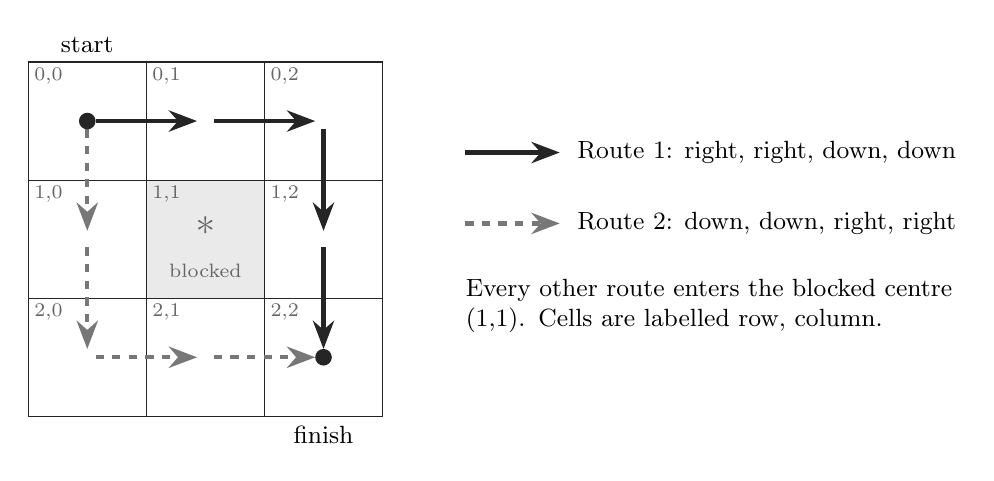
\begin{tikzpicture}[>=Stealth,every node/.style={font=\small},box/.style={draw=teal,rounded corners,minimum width=20mm,minimum height=8mm,fill=wash},arr/.style={->,thick,teal}]\draw[teal,fill=paper] (-0.75,-0.75) rectangle (0.75,0.75);\node[anchor=north west,inner sep=2pt,font=\scriptsize,text=quiet] at (-0.75,0.75) {0,0};\draw[teal,fill=paper] (0.75,-0.75) rectangle (2.25,0.75);\node[anchor=north west,inner sep=2pt,font=\scriptsize,text=quiet] at (0.75,0.75) {0,1};\draw[teal,fill=paper] (2.25,-0.75) rectangle (3.75,0.75);\node[anchor=north west,inner sep=2pt,font=\scriptsize,text=quiet] at (2.25,0.75) {0,2};\draw[teal,fill=paper] (-0.75,-2.25) rectangle (0.75,-0.75);\node[anchor=north west,inner sep=2pt,font=\scriptsize,text=quiet] at (-0.75,-0.75) {1,0};\draw[teal,fill=wash] (0.75,-2.25) rectangle (2.25,-0.75);\node[anchor=north west,inner sep=2pt,font=\scriptsize,text=quiet] at (0.75,-0.75) {1,1};\draw[teal,fill=paper] (2.25,-2.25) rectangle (3.75,-0.75);\node[anchor=north west,inner sep=2pt,font=\scriptsize,text=quiet] at (2.25,-0.75) {1,2};\draw[teal,fill=paper] (-0.75,-3.75) rectangle (0.75,-2.25);\node[anchor=north west,inner sep=2pt,font=\scriptsize,text=quiet] at (-0.75,-2.25) {2,0};\draw[teal,fill=paper] (0.75,-3.75) rectangle (2.25,-2.25);\node[anchor=north west,inner sep=2pt,font=\scriptsize,text=quiet] at (0.75,-2.25) {2,1};\draw[teal,fill=paper] (2.25,-3.75) rectangle (3.75,-2.25);\node[anchor=north west,inner sep=2pt,font=\scriptsize,text=quiet] at (2.25,-2.25) {2,2};\node[font=\Large,text=quiet,inner sep=0pt] at (1.5,-1.4) {*};\node[font=\scriptsize,text=quiet,inner sep=0pt] at (1.5,-1.9) {blocked};\node[anchor=south] at (0,0.75) {start};\node[anchor=north] at (3.0,-3.75) {finish};\draw[arr,line width=1.6pt,shorten >=3pt,shorten <=3pt] (0.0,0.0)--(1.5,0.0);\draw[arr,line width=1.6pt,shorten >=3pt,shorten <=3pt] (1.5,0.0)--(3.0,0.0);\draw[arr,line width=1.6pt,shorten >=3pt,shorten <=3pt] (3.0,0.0)--(3.0,-1.5);\draw[arr,line width=1.6pt,shorten >=3pt,shorten <=3pt] (3.0,-1.5)--(3.0,-3.0);\draw[arr,orange,dashed,line width=1.6pt,shorten >=3pt,shorten <=3pt] (0.0,0.0)--(0.0,-1.5);\draw[arr,orange,dashed,line width=1.6pt,shorten >=3pt,shorten <=3pt] (0.0,-1.5)--(0.0,-3.0);\draw[arr,orange,dashed,line width=1.6pt,shorten >=3pt,shorten <=3pt] (0.0,-3.0)--(1.5,-3.0);\draw[arr,orange,dashed,line width=1.6pt,shorten >=3pt,shorten <=3pt] (1.5,-3.0)--(3.0,-3.0);\fill[teal] (0.0,0.0) circle (3pt);\fill[teal] (3.0,-3.0) circle (3pt);\draw[arr,line width=1.6pt] (4.8,-0.4)--(6.0,-0.4);\node[anchor=west] at (6.1,-0.4) {Route 1: right, right, down, down};\draw[arr,orange,dashed,line width=1.6pt] (4.8,-1.3)--(6.0,-1.3);\node[anchor=west] at (6.1,-1.3) {Route 2: down, down, right, right};\node[anchor=north west,text width=62mm,inner sep=0pt] at (4.8,-2.0) {Every other route enters the blocked centre (1,1). Cells are labelled row, column.};\end{tikzpicture}\end{center}
The first route visits cells (0,0), (0,1), (0,2), (1,2), (2,2). The second visits (0,0), (1,0), (2,0), (2,1), (2,2). In each pair, the first number is the row and the second is the column. Neither route visits (1,1).

\end{qblock}
\end{qblock}\par\medskip{\color{lightink}\hrule height .4pt}\bigskip
\par\markboth{A grid cell receives two counts}{}\begin{qblock}\begin{qblock}[0.95]
\qtopic{L2-10}{A grid cell receives two counts}
{\small\color{quiet}Grid Paths: count routes to each cell}\par\medskip
\textbf{Question.} Rows and columns are numbered from 0. Let paths[r][c] count routes from the top-left cell to row r, column c. From which cells can the last move arrive? Fill the count table for the 3 by 3 grid with its centre blocked, writing 0 for the blocked cell.

\textbf{Table supplied with the question.}\par\par\medskip \begingroup\small\setlength{\tabcolsep}{4pt}\renewcommand{\arraystretch}{1.35}\begin{tabularx}{\linewidth}{>{\raggedright\arraybackslash}X>{\raggedright\arraybackslash}X>{\raggedright\arraybackslash}X>{\raggedright\arraybackslash}X}\toprule\textbf{Row / column} & \textbf{0} & \textbf{1} & \textbf{2}\\\midrule
0 & 1 & ? & ?\\
1 & ? & ? & ?\\
2 & ? & ? & ?\\
\bottomrule\end{tabularx}\endgroup\par\medskip 
\par\medskip\textbf{Worked answer.} An open cell receives paths from above and from its left. The count table is rows [1, 1, 1], [1, 0, 1], [1, 1, 2]. A blocked cell contributes zero.

\textbf{Completed table.}\par\par\medskip \begingroup\small\setlength{\tabcolsep}{4pt}\renewcommand{\arraystretch}{1.35}\begin{tabularx}{\linewidth}{>{\raggedright\arraybackslash}X>{\raggedright\arraybackslash}X>{\raggedright\arraybackslash}X>{\raggedright\arraybackslash}X}\toprule\textbf{Row / column} & \textbf{0} & \textbf{1} & \textbf{2}\\\midrule
0 & 1 & 1 & 1\\
1 & 1 & 0 & 1\\
2 & 1 & 1 & 2\\
\bottomrule\end{tabularx}\endgroup\par\medskip 
The open start stores 1 for the empty path. At row 1, column 2, the cell above contributes 1 and the blocked cell to the left contributes 0: 1 + 0 = 1. At the bottom right, above and left contribute 1 each, giving 2.

\end{qblock}
\end{qblock}\par\medskip{\color{lightink}\hrule height .4pt}\bigskip
\par\markboth{Grid recursion identifies a cell}{}\begin{qblock}\begin{qblock}[0.95]
\qtopic{L2-11}{Grid recursion identifies a cell}
{\small\color{quiet}Grid Paths: count routes to each cell}\par\medskip
\textbf{Question.} Write grid\_cached(rows) with a cached recursive helper count(r, c). The helper returns the number of legal paths from the top-left cell to cell (r, c). Ask about the cells above and to the left. State the answers for an outside cell, a blocked cell and an open starting cell. Why do the calls stop?

\par\smallskip{\small\textbf{Start with:}}\par\smallskip\noindent\colorbox{codepaper}{\parbox{\dimexpr\linewidth-2\fboxsep\relax}{\small\ttfamily\raggedright def grid\_cached(rows):\\\hspace*{2.4em}n = len(rows)\\\hspace*{2.4em}def count(r, c):\\\hspace*{4.8em}return None  \# Your helper goes here.\\\hspace*{2.4em}return count(n - 1, n - 1)}}\par
{\small\textbf{What each function returns.}\par grid\_cached(rows): the number of legal paths from top-left to bottom-right, modulo 1,000,000,007.\par count(r, c): the number of legal paths from top-left to cell (r, c), modulo 1,000,000,007.\par }
{\small\textbf{Hints.}}\begin{itemize}\item Which cells can you answer directly: outside the grid, blocked, and the start?\item From which two cells can the last move into (r, c) come?\end{itemize}
\par\medskip\textbf{Worked answer.} The key is the pair (r, c). Each call goes one row up or one column left, so r + c decreases. Outside cells and blocked cells return 0; the open starting cell returns 1.

\end{qblock}
\begin{qblock}[0.95]
\medskip\textbf{One complete Python implementation: grid\_cached.}\label{ans-grid_cached}\par
\begin{lstlisting}[style=numbered]
from functools import lru_cache

MOD = 1_000_000_007

def grid_cached(rows):
    n = len(rows)
    @lru_cache(None)
    def count(r, c):
        if r < 0 or c < 0 or rows[r][c] == '*':
            return 0
        if r == 0 and c == 0:
            return 1
        return (count(r - 1, c) + count(r, c - 1)) % MOD
    return count(n - 1, n - 1)
\end{lstlisting}
\textbf{Check.} Run this after the function above.
\begin{lstlisting}
print(grid_cached(['...', '.*.', '...']))
\end{lstlisting}
\textbf{Expected output.}
\begin{lstlisting}[language={}]
2
\end{lstlisting}
\textbf{Recursion depth.} Python stops recursion at about 1,000 nested calls by default, so this recursive version is for small inputs and the small and edge test files only. Use the iterative version for the medium and large files.

\end{qblock}
\end{qblock}\par\medskip{\color{lightink}\hrule height .4pt}\bigskip
\par\markboth{Grid iteration and independent rows}{}\begin{qblock}\begin{qblock}[0.95]
\qtopic{L2-12}{Grid iteration and independent rows}
{\small\color{quiet}Grid Paths: count routes to each cell}\par\medskip
\textbf{Question.} Write grid\_table(rows) using loops over rows and columns. The grid has n rows and n columns. Fill paths[r][c], taking counts modulo 1,000,000,007. Why does [[0] * n for \_ in range(n)] create independent rows? For n = 2, show what goes wrong with [[0] * n] * n when one cell changes.

\par\smallskip{\small\textbf{Start with:}}\par\smallskip\noindent\colorbox{codepaper}{\parbox{\dimexpr\linewidth-2\fboxsep\relax}{\small\ttfamily\raggedright def grid\_table(rows):\\\hspace*{2.4em}return None  \# Replace with your answer.}}\par
{\small\textbf{What each function returns.}\par grid\_table(rows): the number of legal paths from top-left to bottom-right, modulo 1,000,000,007.\par }
{\small\textbf{Hints.}}\begin{itemize}\item Create the table so that every row is a separate list.\item In which order must you visit the cells so that the cells above and to the left are already filled?\item What does a blocked cell store?\end{itemize}
\par\medskip\textbf{Worked answer.} A comprehension builds a new list for each row. With bad = [[0] * 2] * 2, setting bad[0][0] = 1 makes both rows [1, 0], because they share one list. Separate rows keep the second row unchanged. Fill each open cell from above and left, then return the bottom-right count.

For the incorrect construction, bad = [[0] * 2] * 2 repeats references to one row. After bad[0][0] = 1, the grid is [[1, 0], [1, 0]]. A comprehension instead creates two rows, so the same assignment gives [[1, 0], [0, 0]].

\end{qblock}
\begin{qblock}[0.95]
\medskip\textbf{One complete Python implementation: grid\_table.}\label{ans-grid_table}\par
\begin{lstlisting}[style=numbered]
MOD = 1_000_000_007

def grid_table(rows):
    n = len(rows)
    paths = [[0] * n for _ in range(n)]
    for r in range(n):
        for c in range(n):
            if rows[r][c] == '*':
                continue
            if r == 0 and c == 0:
                paths[r][c] = 1
            else:
                above = paths[r - 1][c] if r > 0 else 0
                left = paths[r][c - 1] if c > 0 else 0
                paths[r][c] = (above + left) % MOD
    return paths[-1][-1]
\end{lstlisting}
\textbf{Check.} Run this after the function above.
\begin{lstlisting}
print(grid_table(['...', '.*.', '...']))
\end{lstlisting}
\textbf{Expected output.}
\begin{lstlisting}[language={}]
2
\end{lstlisting}
\end{qblock}
\end{qblock}\par\medskip{\color{lightink}\hrule height .4pt}\bigskip
\par\markboth{Your turn: test the boundaries}{}\begin{qblock}\begin{qblock}[0.95]
\qtopic{L2-13}{Your turn: test the boundaries}
{\small\color{quiet}Grid Paths: count routes to each cell}\par\medskip
\textbf{Question.} Test your grid\_table(rows) from L2-12. First predict the answers for a single open cell, a single blocked cell, an open 2 by 2 grid, and a 3 by 3 grid with the centre blocked. Then run your function and compare.

\textbf{Table supplied with the question.}\par\par\medskip \begingroup\small\setlength{\tabcolsep}{4pt}\renewcommand{\arraystretch}{1.35}\begin{tabularx}{\linewidth}{>{\raggedright\arraybackslash}X>{\raggedright\arraybackslash}X>{\raggedright\arraybackslash}X}\toprule\textbf{Test grid} & \textbf{Your prediction} & \textbf{Program output}\\\midrule
{}['.']  (one open cell) &  & \\
{}['*']  (one blocked cell) &  & \\
{}['..', '..']  (open 2 by 2) &  & \\
{}['...', '.*.', '...']  (centre blocked) &  & \\
\bottomrule\end{tabularx}\endgroup\par\medskip 
\par\medskip\textbf{Worked answer.} The answers are 1, 0, 2 and 2 respectively. An open start has one empty route. A blocked start has none. In the 2 by 2 grid the routes are right-down and down-right.

\textbf{Completed table.}\par\par\medskip \begingroup\small\setlength{\tabcolsep}{4pt}\renewcommand{\arraystretch}{1.35}\begin{tabularx}{\linewidth}{>{\raggedright\arraybackslash}X>{\raggedright\arraybackslash}X>{\raggedright\arraybackslash}X}\toprule\textbf{Test grid} & \textbf{Your prediction} & \textbf{Program output}\\\midrule
{}['.']  (one open cell) & 1 & 1\\
{}['*']  (one blocked cell) & 0 & 0\\
{}['..', '..']  (open 2 by 2) & 2 & 2\\
{}['...', '.*.', '...']  (centre blocked) & 2 & 2\\
\bottomrule\end{tabularx}\endgroup\par\medskip 
\end{qblock}
\begin{qblock}[0.95]
\medskip\textbf{Same implementation as L2-12} (\texttt{grid\_table}, page~\pageref{ans-grid_table}).\par\textbf{Check.} Run this after that function.
\begin{lstlisting}
for grid in [['.'], ['*'], ['..', '..'], ['...', '.*.', '...']]:
    print(grid_table(grid))
\end{lstlisting}
\textbf{Expected output.}
\begin{lstlisting}[language={}]
1
0
2
2
\end{lstlisting}
\end{qblock}
\end{qblock}\par\medskip{\color{lightink}\hrule height .4pt}\bigskip
\par\markboth{The shared counting idea}{}\begin{qblock}\begin{qblock}[0.95]
\qtopic{L2-14}{The shared counting idea}
{\small\color{quiet}Grid Paths: count routes to each cell}\par\medskip
\textbf{Question.} In Dice, group completed sequences by their last number. In Grid Paths, group completed paths by their last move. Why can we add the group counts in each problem? Explain why no completed sequence or path belongs to two of these groups.

\par\medskip\textbf{Worked answer.} Both describe the last move of a completed object. Each valid sequence or path belongs to exactly one last-move group. Add those groups when they are exhaustive and do not overlap.

A dice sequence has one final face, even when earlier faces repeat. A nonempty grid path has one final move: right or down. Removing that last choice gives the earlier sequence or path counted by the recurrence. The empty sequence and the open starting cell are handled by the base answer 1.

\end{qblock}
\end{qblock}\par\medskip{\color{lightink}\hrule height .4pt}\bigskip
\end{document}